\documentclass{ximera}

\usepackage[T1]{fontenc}
\usepackage{stix2}
\usepackage{gillius}
\usepackage{resizegather}
%\usepackage{rsfso} fancy cal
\DeclareMathAlphabet{\mathcal}{OMS}{cmsy}{m}{n} %less fancy cal


\usepackage{multicol}


\usepackage{tikz-cd}
\usepackage{tkz-euclide} %% compass
\usetkzobj{all}  %% tkzCompass
\tikzset{>=stealth}
\tikzcdset{arrow style=tikz}
\usetikzlibrary{math} %% for assigning variables
%\usetikzlibrary{fadings}

\usepackage{colortbl,boldline,makecell} %% group tables


\usepackage[sans]{dsfont}

\usepackage{stmaryrd,pifont}

\graphicspath{
  {./}
  {fields/}
  }     



\let\oldbibliography\thebibliography%% to compact bib
\renewcommand{\thebibliography}[1]{%
  \oldbibliography{#1}%
  \setlength{\itemsep}{0pt}%
}
\renewcommand\refname{} %% no name needed!


\DefineVerbatimEnvironment{macaulay2}{Verbatim}{numbers=left,frame=lines,label=Macaulay2,labelposition=topline}

\DefineVerbatimEnvironment{gap}{Verbatim}{numbers=left,frame=lines,label=GAP,labelposition=topline}

%%% This next bit of code defines all our theorem environments
\makeatletter
\let\c@theorem\relax
\let\c@corollary\relax
%\let\c@example\relax
\makeatother

\let\definition\relax
\let\enddefinition\relax

\let\theorem\relax
\let\endtheorem\relax

\let\proposition\relax
\let\endproposition\relax

\let\exercise\relax
\let\endexercise\relax

\let\question\relax
\let\endquestion\relax

\let\remark\relax
\let\endremark\relax

\let\corollary\relax
\let\endcorollary\relax


\let\example\relax
\let\endexample\relax

\let\warning\relax
\let\endwarning\relax

\let\lemma\relax
\let\endlemma\relax


\let\algorithm\relax
\let\endalgorithm\relax
\usepackage{algpseudocode}

\newtheoremstyle{SlantTheorem}{\topsep}{\topsep}%%% space between body and thm
		{\slshape}                      %%% Thm body font
		{}                              %%% Indent amount (empty = no indent)
		{\bfseries\sffamily}            %%% Thm head font
		{}                              %%% Punctuation after thm head
		{3ex}                           %%% Space after thm head
		{\thmname{#1}\thmnumber{ #2}\thmnote{ \bfseries(#3)}}%%% Thm head spec
\theoremstyle{SlantTheorem}
\newtheorem{theorem}{Theorem}
%\newtheorem{definition}[theorem]{Definition}
%\newtheorem{proposition}[theorem]{Proposition}
%% \newtheorem*{dfnn}{Definition}
%% \newtheorem{ques}{Question}[theorem]
%% \newtheorem*{war}{WARNING}
%% \newtheorem*{cor}{Corollary}
%% \newtheorem*{eg}{Example}
\newtheorem*{remark}{Remark}
\newtheorem*{touchstone}{Touchstone}
\newtheorem{corollary}{Corollary}[theorem]
\newtheorem*{warning}{WARNING}
\newtheorem{example}[corollary]{Example}
\newtheorem{lemma}[theorem]{Lemma}




\newtheoremstyle{Definition}{\topsep}{\topsep}%%% space between body and thm
		{}                              %%% Thm body font
		{}                              %%% Indent amount (empty = no indent)
		{\bfseries\sffamily}            %%% Thm head font
		{}                              %%% Punctuation after thm head
		{3ex}                           %%% Space after thm head
		{\thmname{#1}\thmnumber{ #2}\thmnote{ \bfseries(#3)}}%%% Thm head spec
\theoremstyle{Definition}
\newtheorem{definition}[theorem]{Definition}



\let\algorithm\relax
\let\endalgorithm\relax
\newtheoremstyle{Alg}{\topsep}{\topsep}%%% space between body and thm
		{}                              %%% Thm body font
		{}                              %%% Indent amount (empty = no indent)
		{\bfseries\sffamily}            %%% Thm head font
		{}                              %%% Punctuation after thm head
		{3ex}                           %%% Space after thm head
		{\thmname{#1}\thmnumber{ #2}\thmnote{ \bfseries(#3)}}%%% Thm head spec
\theoremstyle{Alg}
\newtheorem*{algorithm}{Algorithm}
\newtheorem*{construction}{Construction}




\newtheoremstyle{Exercise}{\topsep}{\topsep} %%% space between body and thm
		{}                           %%% Thm body font
		{}                           %%% Indent amount (empty = no indent)
		{\bfseries\sffamily}         %%% Thm head font
		{)}                          %%% Punctuation after thm head
		{ }                          %%% Space after thm head
		{\thmnumber{#2}\thmnote{ \bfseries(#3)}}%%% Thm head spec
\theoremstyle{Exercise}
\newtheorem{exercise}[corollary]{}%[theorem]

%% \newtheoremstyle{Question}{\topsep}{\topsep} %%% space between body and thm
%% 		{\bfseries}                  %%% Thm body font
%% 		{3ex}                        %%% Indent amount (empty = no indent)
%% 		{}                           %%% Thm head font
%% 		{}                           %%% Punctuation after thm head
%% 		{}                           %%% Space after thm head
%% 		{\thmnumber{#2}\thmnote{ \bfseries(#3)}}%%% Thm head spec
\newtheoremstyle{Question}{3em}{3em} %%% space between body and thm
		{\large\bfseries}                           %%% Thm body font
		{}                           %%% Indent amount (empty = no indent)
		{}                         %%% Thm head font
		{}                          %%% Punctuation after thm head
		{0em}                          %%% Space after thm head
		{}%%% Thm head spec
\theoremstyle{Question}
\newtheorem*{question}{}






\renewcommand{\tilde}{\widetilde}
\renewcommand{\bar}{\overline}
\renewcommand{\hat}{\widehat}
\newcommand{\N}{\mathbb N}
\newcommand{\Z}{\mathbb Z}
\newcommand{\R}{\mathbb R}
\newcommand{\Q}{\mathbb Q}
\newcommand{\C}{\mathbb C}
\newcommand{\V}{\mathbb V}
\newcommand{\I}{\mathbb I}
\newcommand{\A}{\mathbb A}
\renewcommand{\o}{\mathbf o}
\newcommand{\iso}{\simeq}
\newcommand{\ph}{\varphi}
\newcommand{\Cf}{\mathcal{C}}
\newcommand{\IZ}{\mathrm{Int}(\Z)}
\newcommand{\dsum}{\oplus}
\newcommand{\directsum}{\bigoplus}
\newcommand{\union}{\bigcup}
\newcommand{\subgp}{\leq}
\newcommand{\normal}{\trianglelefteq}
\renewcommand{\i}{\mathfrak}
\renewcommand{\a}{\mathfrak{a}}
\renewcommand{\b}{\mathfrak{b}}
\newcommand{\m}{\mathfrak{m}}
\newcommand{\p}{\mathfrak{p}}
\newcommand{\q}{\mathfrak{q}}
\newcommand{\dfn}[1]{\textbf{#1}\index{#1}}
\let\hom\relax
\DeclareMathOperator{\mat}{Mat}
\DeclareMathOperator{\ann}{Ann}
\DeclareMathOperator{\h}{ht}
\DeclareMathOperator{\tr}{tr}
\DeclareMathOperator{\hom}{Hom}
\DeclareMathOperator{\Span}{Span}
\DeclareMathOperator{\spec}{Spec}
\DeclareMathOperator{\maxspec}{MaxSpec}
\DeclareMathOperator{\aut}{Aut}
\DeclareMathOperator{\ass}{Ass}
\DeclareMathOperator{\lcm}{lcm}
\DeclareMathOperator{\ff}{Frac}
\DeclareMathOperator{\im}{Im}
\DeclareMathOperator{\syz}{Syz}
\DeclareMathOperator{\gr}{Gr}
\DeclareMathOperator{\multideg}{multideg}
\renewcommand{\ker}{\mathop{\mathrm{Ker}}\nolimits}
\newcommand{\coker}{\mathop{\mathrm{Coker}}\nolimits}
\newcommand{\lps}{[\hspace{-0.25ex}[}
\newcommand{\rps}{]\hspace{-0.25ex}]}
\newcommand{\into}{\hookrightarrow}
\newcommand{\onto}{\twoheadrightarrow}
\newcommand{\tensor}{\otimes}
\newcommand{\x}{\mathbf{x}}
\newcommand{\X}{\mathbf X}
\newcommand{\Y}{\mathbf Y}
\renewcommand{\k}{\boldsymbol{\kappa}}
\renewcommand{\emptyset}{\varnothing}
\renewcommand{\qedsymbol}{$\blacksquare$}
\renewcommand{\l}{\ell}
\newcommand{\1}{\mathds{1}}
\newcommand{\lto}{\mathop{\longrightarrow\,}\limits}
\newcommand{\rad}{\sqrt}
\newcommand{\hf}{H}
\newcommand{\hs}{H\!S}
\newcommand{\hp}{H\!P}
\renewcommand{\vec}{\mathbf}
\let\temp\phi
\let\phi\varphi
\let\eulerphi\temp


\renewcommand{\epsilon}{\varepsilon}
\renewcommand{\subset}{\subseteq}
\renewcommand{\supset}{\supseteq}
\newcommand{\macaulay}{\normalfont\textsl{Macaulay2}}
\newcommand{\GAP}{\normalfont\textsf{GAP}}
\newcommand{\invlim}{\varprojlim}
\renewcommand{\le}{\leqslant}
\renewcommand{\ge}{\geqslant}
\newcommand{\valpha}{{\boldsymbol\alpha}}
\newcommand{\vbeta}{{\boldsymbol\beta}}
\newcommand{\vgamma}{{\boldsymbol\gamma}}
\newcommand{\dotp}{\bullet}
\newcommand{\lc}{\normalfont\textsc{lc}}
\newcommand{\lt}{\normalfont\textsc{lt}}
\newcommand{\lm}{\normalfont\textsc{lm}}
\newcommand{\from}{\leftarrow}
\newcommand{\transpose}{\intercal}
\newcommand{\grad}{\boldsymbol\nabla}
\newcommand{\curl}{\boldsymbol{\nabla\times}}
\renewcommand{\d}{\, d}
\newcommand{\<}{\langle}
\renewcommand{\>}{\rangle}

%\renewcommand{\proofname}{Sketch of Proof}


\renewenvironment{proof}[1][Proof]
  {\begin{trivlist}\item[\hskip \labelsep \itshape \bfseries #1{}\hspace{2ex}]\upshape}
{\qed\end{trivlist}}

\newenvironment{sketch}[1][Sketch of Proof]
  {\begin{trivlist}\item[\hskip \labelsep \itshape \bfseries #1{}\hspace{2ex}]\upshape}
{\qed\end{trivlist}}



\makeatletter
\renewcommand\section{\@startsection{paragraph}{10}{\z@}%
                                     {-3.25ex\@plus -1ex \@minus -.2ex}%
                                     {1.5ex \@plus .2ex}%
                                     {\normalfont\large\sffamily\bfseries}}
\renewcommand\subsection{\@startsection{subparagraph}{10}{\z@}%
                                    {3.25ex \@plus1ex \@minus.2ex}%
                                    {-1em}%
                                    {\normalfont\normalsize\sffamily\bfseries}}
\makeatother

%% Fix weird index/bib issue.
\makeatletter
\gdef\ttl@savemark{\sectionmark{}}
\makeatother


\makeatletter
%% no number for refs
\newcommand\frontstyle{%
  \def\activitystyle{activity-chapter}
  \def\maketitle{%
    \addtocounter{titlenumber}{1}%
                    {\flushleft\small\sffamily\bfseries\@pretitle\par\vspace{-1.5em}}%
                    {\flushleft\LARGE\sffamily\bfseries\@title \par }%
                    {\vskip .6em\noindent\textit\theabstract\setcounter{problem}{0}\setcounter{sectiontitlenumber}{0}}%
                    \par\vspace{2em}
                    \phantomsection\addcontentsline{toc}{section}{\textbf{\@title}}%
                  }}
\makeatother



\NewEnviron{annotate}{\vspace{-.3cm}\small \itshape \BODY \vspace{.3cm}}


%%%% TIKZ STUFF

%% N-GON code
\tikzset{
    pics/tikzngon/.style={
        code={
        \tikzmath{\xx = #1;\rr=1.7;}
        \draw[ultra thick,rounded corners=.05mm] ({\rr*sin(0*360/\xx)},{\rr*cos(0*360/\xx)})
        \foreach \x in {-1,0,...,\xx}
        {
        -- ({\rr*sin(\x*360/\xx)},{\rr*cos(\x*360/\xx)})
        }
           -- cycle;
  }}}

%% N-GON code (even)
\tikzset{
    pics/tikzegon/.style={
        code={
        \tikzmath{\xx = #1;\rr=1.7;}
        \draw[ultra thick,rounded corners=.05mm] ({\rr*sin(0*360/\xx+180/\xx)},{\rr*cos(0*360/\xx+180/\xx)})
        \foreach \x in {-1,0,...,\xx}
           {
           -- ({\rr*sin(\x*360/\xx+180/\xx)},{\rr*cos(\x*360/\xx+180/\xx)}) 
           }
           -- cycle;
  }}}




%% N-CLOCK code
\tikzset{
    pics/tikznclock/.style={
        code={
        \tikzmath{\xx = #1;\rr=1.7;\dd=.4;}
        \foreach \x in {1,...,\xx}
        \pgfmathtruncatemacro{\xy}{\x-1}
           {
             \node[circle,fill=black,inner sep=0pt, minimum size=13pt,text=white]
             at ({(\rr-\dd)*sin((\x-1)*360/(\xx)},{(\rr-\dd)*cos((\x-1)*360/\xx}) {\normalfont\bfseries\sffamily\small {\xy}};
           }
  \draw[thick] (0,0) circle (\rr);
  }}}



%% barcode from
%% https://tex.stackexchange.com/questions/6895/is-there-a-good-latex-package-for-generating-barcodes
%% NOT CURRENTLY USED!


\def\barcode#1#2#3#4#5#6#7{\begingroup%
  \dimen0=0.1em
  \def\stack##1##2{\oalign{##1\cr\hidewidth##2\hidewidth}}%
  \def\0##1{\kern##1\dimen0}%
  \def\1##1{\vrule height10ex width##1\dimen0}%
  \def\L##1{\ifcase##1\bc3211##1\or\bc2221##1\or\bc2122##1\or\bc1411##1%
    \or\bc1132##1\or\bc1231##1\or\bc1114##1\or\bc1312##1\or\bc1213##1%
    \or\bc3112##1\fi}%
  \def\R##1{\bgroup\let\next\1\let\1\0\let\0\next\L##1\egroup}%
  \def\G##1{\bgroup\let\bc\bcg\L##1\egroup}% reverse
  \def\bc##1##2##3##4##5{\stack{\0##1\1##2\0##3\1##4}##5}%
  \def\bcg##1##2##3##4##5{\stack{\0##4\1##3\0##2\1##1}##5}%
  \def\bcR##1##2##3##4##5##6{\R##1\R##2\R##3\R##4\R##5\R##6\11\01\11\09%
    \endgroup}%
  \stack{\09}#1\11\01\11\L#2%
  \ifcase#1\L#3\L#4\L#5\L#6\L#7\or\L#3\G#4\L#5\G#6\G#7%
    \or\L#3\G#4\G#5\L#6\G#7\or\L#3\G#4\G#5\G#6\L#7%
    \or\G#3\L#4\L#5\G#6\G#7\or\G#3\G#4\L#5\L#6\G#7%
    \or\G#3\G#4\G#5\L#6\L#7\or\G#3\L#4\G#5\L#6\G#7%
    \or\G#3\L#4\G#5\G#6\L#7\or\G#3\G#4\L#5\G#6\L#7%
  \fi\01\11\01\11\01\bcR}


\author{Bart Snapp}

\title{Polynomials, degree, and roots}

\begin{document}
\begin{abstract}
  We view sets of polynomials as a vector space over a field.
\end{abstract}
\maketitle


\begin{definition}\index{degree!of a polynomial}
  Let $K$ be a field. A \dfn{polynomial} over $K$, is a formal sum
  \[
  f = c_nx^n + c_{n-1}x^{n-1} + \dots + c_1 x + c_0
  \]
  where $n$ is a nonnegative integer and each $c_i \in K$. The number
  $n$ is the \textbf{degree} of the polynomial, $\deg(f) = n$, and the
  field element $c_n$ is the \dfn{leading coefficient}. If $f=0$, we
  leave the degree of $f$ undefined. The set of all polynomials in
  terms of $x$ with coefficients in $K$ is denoted $K[x]$.\index{K[x]@$K[x]$}
\end{definition}

\begin{exercise} 
  Which of the following are polynomials in $\R[x]$?
  \begin{selectAll}
    \choice[correct]{$f(x) = 0$}
    \choice[correct]{$f(x) = -9$}
    \choice[correct]{$f(x) = 3x+1$}
    \choice{$f(x) = x^{1/2}-x +8$}
    \choice{$f(x) = -4x^{-3}+5x^{-1}+7-18x^2$}
    \choice{$f(x) = \frac{x^2 - 3x + 2}{x-2}$}
    \choice[correct]{$f(x) = x^7-32x^6-\pi x^3+45/84$}
  \end{selectAll}
\end{exercise}


\begin{exercise}
  Prove that if $f,g\in K[x]$ are nonzero, then
  \begin{align*}
    \deg(f+g) &\le \max\{\deg(f),\deg(g)\}\\
    \deg(f\cdot g) &= \deg(f) + \deg(g).
  \end{align*}
\end{exercise}



\begin{definition}
  Let $K$ be a field and $f= c_nx^n + \dots + c_1 x+ c_0$ be a
  polynomial in $K[x]$. An element $\alpha\in K$ is a \dfn{root} of
  $f$ if
  \[
  c_n\alpha^n + \dots + c_1 \alpha+ c_0 =0.
  \]
\end{definition}


Roots have a strong connection to reducibility.


\begin{theorem}[Polynomial division theorem]\label{T:divThmPoly}
\index{division theorem}

Let $K$ be a field and consider any polynomial $n(x)\in K[x]$ and a
nonzero polynomial $d(x)$. Then there exist unique polynomials $q(x)$
and $r(x)$ such that
\[
n(x) = d(x) q(x) + r(x) \qquad \text{with $r(x) = 0$ or $\deg(r) <
  \deg(d)$}.
\]
\begin{sketch}
  We will prove that the quotient and remainder in the polynomial
  division theorem exist.
\begin{enumerate}
\item Prove the existence of $q(x)$ and $r(x)$ if $\deg(n(x))=0$.
\item Prove the existence of $q(x)$ and $r(x)$ if $d(x)|n(x)$.
\item Suppose that $\deg(n(x)) \ne 0$ and $d(x)\nmid n(x)$. Consider the set:
\[
\mathcal{S} = \{1+\deg(n(x) -  d(x)f(x)) : f(x)\in K[x]\}
\]
Explain why $\mathcal S$ is not empty.
\item Explain why $\mathcal S$ has a least element.
\item Use the least element found above to obtain an element $r(x)$
  and explain why $\deg(r(x)) < \deg(d(x))$. Hint, suppose that $\deg(r)\ge
  \deg(d)$ and consider the polynomial
  \[
  s(x) = r(x) - cx^{\deg(r)-\deg(d)} \cdot d(x)
  \]
  for some suitable value of $c$.
\item Explain how to choose $q(x)$ satisfying the conditions of the
  polynomial division theorem.
\end{enumerate}

Now we will prove that the quotient and remainder in the polynomial
division theorem are unique.
\begin{enumerate}
\item Suppose that $(q_1(x),r_1(x))$ and $(q_2(x),r_2(x))$ both satisfied the
  conditions of the theorem for a divisor $n(x)$ and dividend
  $d(x)$. Use these two equations to produce a third equation relating
  $d(x)$, $q_1(x)$, $q_2(x)$, $r_1(x)$, and $r_2(x)$.
\item If $q_1(x) \ne q_2(x)$ explain why $\deg(r_1(x) - r_2(x)) \ge \deg(d(x))$.
\end{enumerate}
\end{sketch}
\end{theorem}

\begin{corollary}[Roots and linear factors]\label{C:rlf}
  If $f(x)\in K[x]$ and $\alpha\in K$, then there exists unique $q(x)\in
  K[x]$ such that
  \[
  f(x) = (x-\alpha)\cdot q(x) + f(\alpha)
  \]
\end{corollary}

This corollary says that if $\alpha$ is a root of $f\in K[x]$, then
\[
(x-\alpha) | f(x).
\]
This is a critical insight.


\begin{definition}
  Let $K$ be a field, and $f(x)\in K[x]$ with $\deg(f(x))>0$. The
  polynomial $f(x)$ is \dfn{irreducible} in $K[x]$ if $f(x)$ cannot be
  expressed as the product of polynomials in $K[x]$ of positive
  degree.
\end{definition}

\begin{example}[Irreducible polynomials]\hfil
  \begin{itemize}
  \item The polynomial $x$ is irreducible in $\C[x]$.
  \item The polynomial $x^2+1$ is irreducible in $\R[x]$, but not in
    $\C[x]$.
  \item The polynomial $x^2-2$ is irreducible in $\Q[x]$, but not in
    $\R[x]$ or $\C[x]$.
  \end{itemize}
\end{example}

\begin{corollary}[Roots of irreducible polynomials]
  Let $K$ be a field. An irreducible polynomial $f(x)$ has a root in
  $K$ if and only if $\deg(f(x))= 1$.
  \begin{sketch}
    $(\Rightarrow)$ Suppose that $f(x)$ is irreducible in $K[x]$ and
    it has a root, $\alpha\in K$. We must show that $\deg(f(x))=
    1$. By Corollary~\ref{C:rlf}, we may write
    \[
    f(x) = (x-\alpha)\cdot q(x)\qquad\deg(q(x))< 1
    \]
    where $q(x)\in K[x]$. But this means $\deg(q(x)) = 0$, and so
    $f(x) = (x-\alpha)\cdot c$, a polynomial of degree one.


    $(\Leftarrow)$ Simply solve a linear equation.
  \end{sketch}
\end{corollary}

\begin{exercise}
  List all irreducible polynomials in $\Z_2[x]$ of degree $2$.
\end{exercise}

\begin{exercise}
  List all irreducible polynomials in $\Z_2[x]$ of degree $3$.
\end{exercise}




\begin{theorem}[Degree and roots]
  A polynomial of degree $n$ over a field $K$ has at most $n$ roots.
  \begin{sketch}
    Induction on the degree.
  \end{sketch}
\end{theorem}

\begin{remark}
  Note, in the theorem above it was critical that $K$ is a
  field. Consider $x^2+1$ in $Q_8$, this polynomial has three
  distinct roots!
\end{remark}



\begin{theorem}[The multiplicative group is cyclic]\label{T:mgc}
  Let $K$ be a finite field. In this case, $K^\times = K-\{0\}$ is a
  cyclic group.
  \begin{proof}
    Seeking a contradiction, suppose that $K^\times$ is not
    cyclic. Choose a cyclic subgroup $\< m\> \subgp K^\times$ of
    maximal order. Suppose that $a\notin\<m\>$. By
    Corollary~\ref{C:odmo}, $\o(a)|\o(m)$. Thus there is $q$ such that
    \[
    \o(m) = \o(a)\cdot q.
    \]
    Now consider the polynomial
    \[
    f(x) = x^{\o(m)}-1.
    \]
    every element of $\<m\>$ is a root of $f$ as
    \begin{align*}
    f(m^n) &=  (m^n)^{\o(m)} - 1\\
    &= (m^{\o(m)})^n-1\\
    &= 1^n-1\\
    &=0.
    \end{align*}
    Moreover, every element of $\<a\>$ is a root of $f$ as
    \begin{align*}
    f(a^n) &=  (a^n)^{\o(m)} - 1\\
    &= (a^{\o(m)})^n-1\\
    &= (a^{\o(a)q})^n-1\\
    &= (a^{\o(a)})^{qn}-1\\
    &= 1^{qn}-1\\
    &=0.
    \end{align*}
    But now, $f$ has more than $\o(m)$ roots, a contradiction.
  \end{proof}
\end{theorem}

\begin{corollary}[$\boldsymbol{\pmb\Z_p^{\pmb\times}}$ is cyclic.]\label{C:mzpc}
  The group $\Z_p^\times$ is cyclic.
\end{corollary}









\begin{theorem}[Fundamental theorem of algebra]\index{fundamental theorem of algebra}\label{T:fta}
  Every nonconstant polynomial in $\C[z]$ has at least one root in
  $\C$.
  \begin{sketch}
    We will sketch Gauss' first proof of the fundamental theorem of
    algebra. Suppose you have a polynomial in $\C[z]$,
    \[
    f(z) = c_n z^n + c_{n-1}z^{n-1} + \dots + c_1 z + c_0.
    \]
    In this case $z = x + yi$ where $x,y,\in\R$. Now make two new
    functions of two variables:
    \begin{align*}
      G(x,y) &= \Re(f(x+ yi)) & & \text{(real part of $f(z)$)}\\
      H(x,y) &= \Im(f(x+yi)) & & \text{(imaginary part of $f(z)$)}
    \end{align*}

    Consider the level curves
    \[
    G(x,y) = 0 \quad\text{and}\quad H(x,y) = 0.
    \]
    If these level curves intersect at some point $(x,y)$, then
    $f(x+yi) = 0$. Understanding these level curves precisely is
    difficult. However, if $x$ and $y$ are sufficiently large, then
    \[
    f(z) \approx c_n z^n.
    \]
    It can be shown that if $f(z) = z^n$ then the level curves
    \[
    G(x,y) = 0 \quad\text{and}\quad H(x,y) = 0,
    \]
    are simply lines though the origin:
    \[
    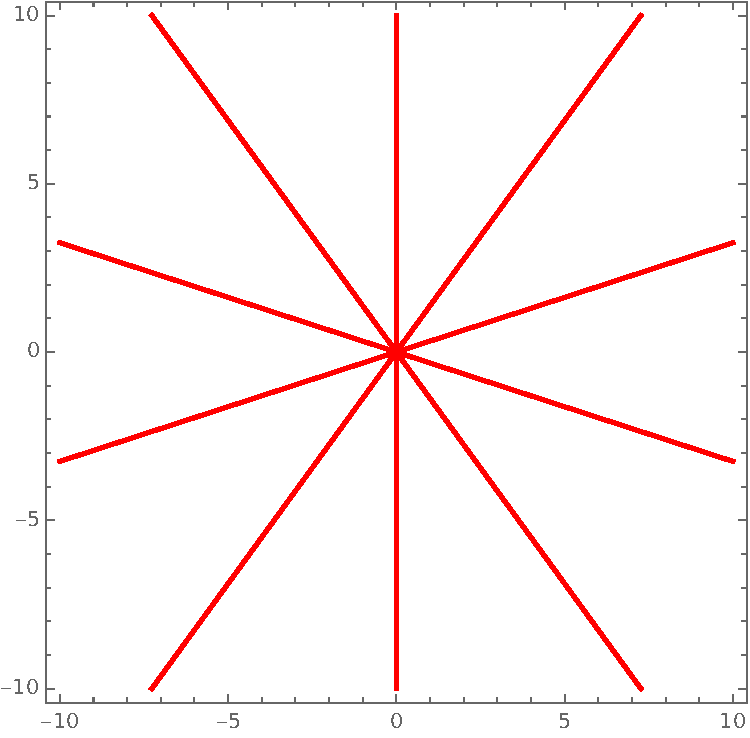
\includegraphics[width=.3\textwidth]{realLines.pdf} \qquad 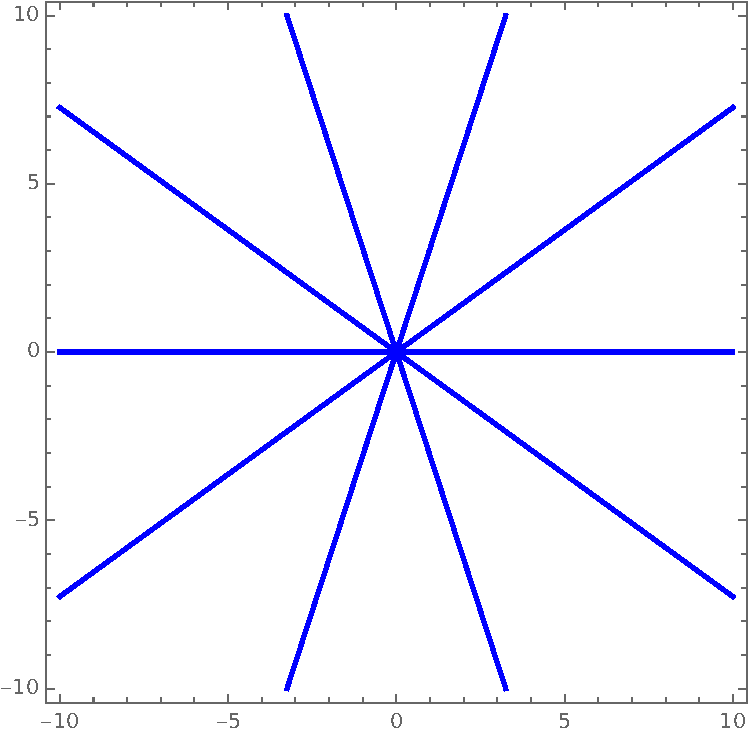
\includegraphics[width=.3\textwidth]{imLines.pdf}
    \]
    On the left we see the level curves for $G$ and on the right we
    see level curves for $H$. In particular, the lines are interleaved:
    \[
    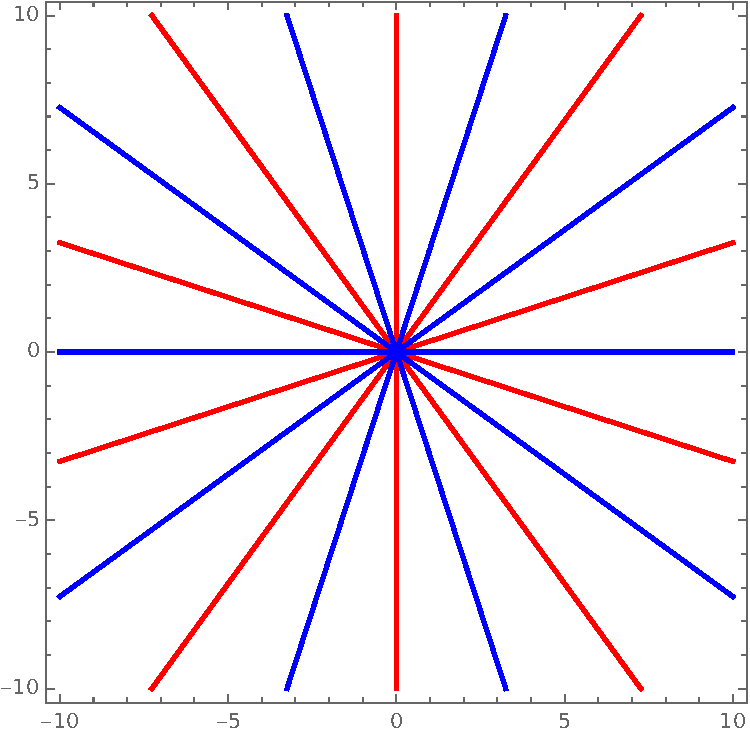
\includegraphics[width=.3\textwidth]{lines.pdf}
    \]
    If you have any polynomial, the level curves will look like this
    for $x$ and $y$ sufficiently large.

    So here is the idea, imagine a circle of very large
    radius. Outside the circle the level curves look like this:
    \[
    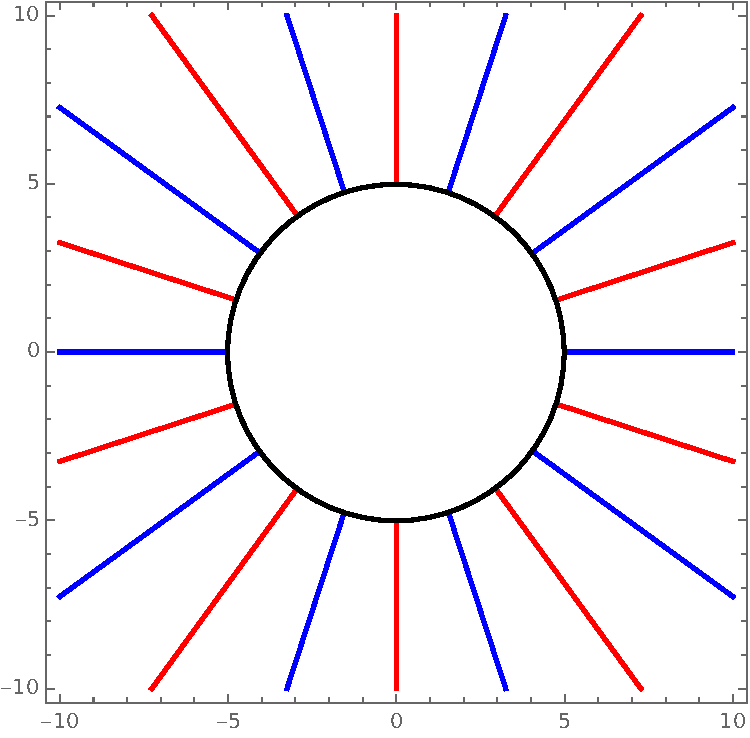
\includegraphics[width=.3\textwidth]{circlelines.pdf}
    \]
    However, we're not real sure what happens inside the circle, so we
    leave it blank.
    
    At this point Gauss claims that any level curve entering the
    circle will leave the circle. This is a hard fact to prove---and
    the source of the gap in Gauss' first proof of the fundamental
    theorem of algebra. Regardless, accepting this fact, we then know
    that the inside of the disk must look something like:
    \[
    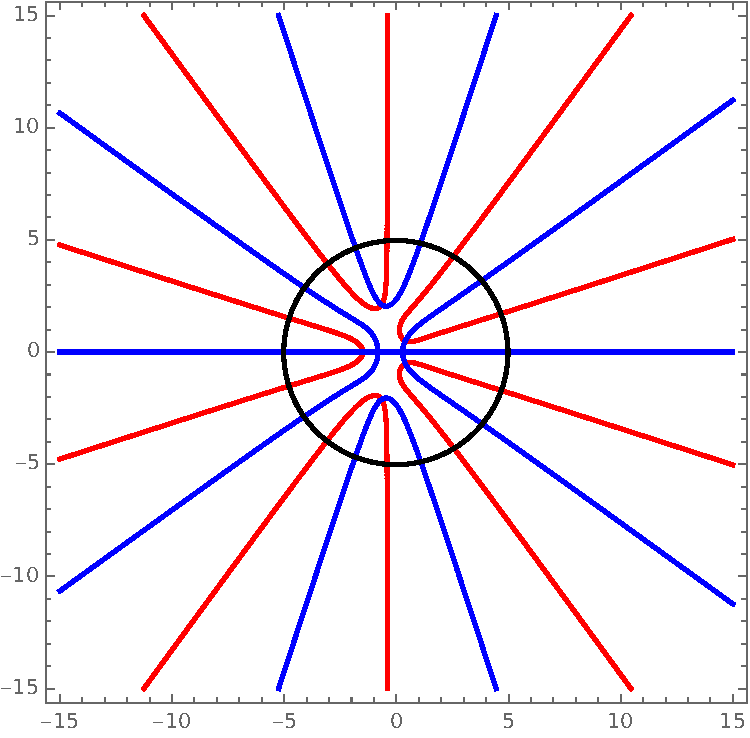
\includegraphics[width=.6\textwidth]{linesIntersection.pdf}
    \]
    Each intersection corresponds to a root in $\C$, and Gauss then
    gave a proof that showed the level curves corresponding to the
    real part and the level curves corresponding to the imaginary part
    must intersect at some point, and hence there is at least one
    complex root.

    In fact, all roots are found that way. For example, above we are
    working with a fifth degree polynomial, and we see we have $5$
    intersections.
  \end{sketch}
\end{theorem}


\begin{remark}
  The proof that we sketched above is actually Gauss' first proof, and
  it was roughly equivalent to Gauss' Ph.D.\ dissertation.
\end{remark}



\begin{corollary}[Irreducible polynomials in $\pmb\C$]
  The only irreducible polynomials in $\C[x]$ are nonconstant linear
  polynomials.
\end{corollary}

\begin{exercise} 
Prove that a polynomial of positive degree $n$ in $\C[x]$ has $n$
(possibly repeated) roots in $\C$.
\end{exercise}


\begin{exercise}\label{E:RQ} 
Show that every polynomial of positive degree in $\R[x]$ can be
factored as a product of polynomials in $\R[x]$ each with degree $1$
or $2$.
\end{exercise}




For some interesting extra reading check out:
\begin{itemize}
\item \link[\textit{On Gauss's first proof of the fundamental theorem of algebra},
  S.\ Basu and D.J.\ Velleman]{https://arxiv.org/abs/1704.06585v1}.
\item \link[\textit{C.F.\ Gauss's proofs of the fundamental theorem of algebra},
  H.\ Cain]{http://math.huji.ac.il/~ehud/MH/Gauss-HarelCain.pdf}.
\item \link[\textit{Cyclicity of $(\Z/(p))^\times$},
  K.\ Conrad]{https://kconrad.math.uconn.edu/blurbs/grouptheory/cyclicmodp.pdf}.
\end{itemize}


\end{document}
